\documentclass[10pt,a4paper]{article}
\usepackage[margin=1.5cm]{geometry}
\usepackage{amsmath,booktabs,tabularx,xcolor,hyperref,enumitem}
\usepackage{tikz}
\usetikzlibrary{positioning,arrows.meta,fit}
\hypersetup{colorlinks,linkcolor=blue!50!black,urlcolor=blue!50!black}
\setlist{itemsep=0pt,topsep=1pt,leftmargin=1.3em}
\pagestyle{empty}
\newcommand{\code}[1]{\texttt{\small #1}}
\definecolor{bad}{HTML}{B5403A}\definecolor{good}{HTML}{2E7D4F}\definecolor{wait}{HTML}{8A6D1F}
\definecolor{spine}{HTML}{2F4F7F}

\begin{document}
\begin{center}
{\Large\bfseries How the methods fit together}\\[2pt]
{\small HY Analyst, 24 October 2026. Section numbers refer to \code{docs/methodology.md}. Page numbers refer to Gatto (2023).}
\end{center}

\noindent\fcolorbox{gray}{gray!6}{\parbox{\dimexpr\linewidth-2\fboxsep-2\fboxrule}{%
\textbf{One idea.} A bond is cheap when its market spread is above the spread its fundamentals justify. Every method does one of two jobs. It builds that fair spread, or it tests a claim that feeds the fair spread. \textbf{Today's state:} the company spine carries the signal. The macro layer failed at all three points where it enters.}}

\medskip
\begin{center}
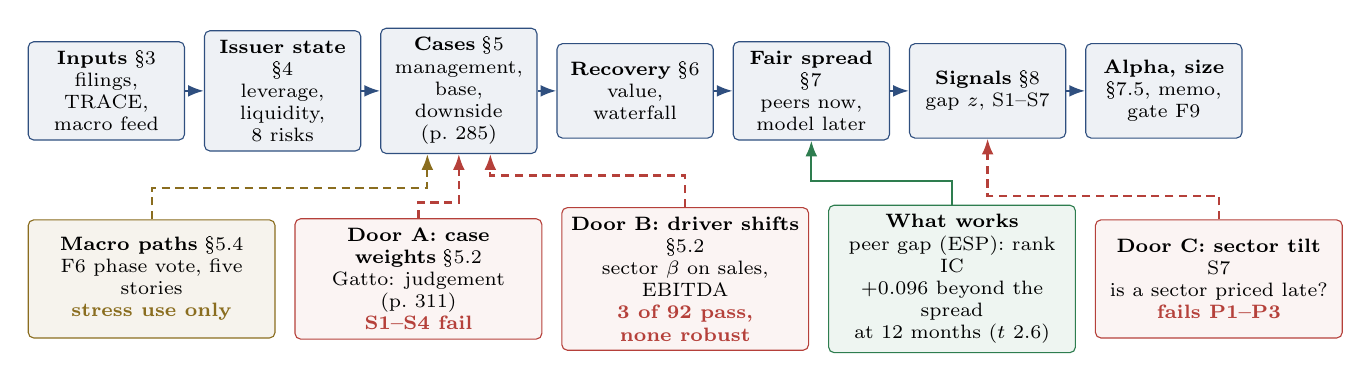
\begin{tikzpicture}[
  node distance=4mm and 2.4mm,
  box/.style={draw=spine,fill=spine!8,rounded corners=2pt,align=flush center,font=\scriptsize,minimum height=12mm,text width=17.5mm},
  door/.style={draw,rounded corners=2pt,align=flush center,font=\scriptsize,text width=29mm,minimum height=15mm},
  marr/.style={-{Latex[length=2mm]},thick,densely dashed,bad}]
\node[box] (in) {\textbf{Inputs} \S3\\filings, TRACE,\\macro feed};
\node[box,right=of in] (st) {\textbf{Issuer state} \S4\\leverage, liquidity,\\8 risks};
\node[box,right=of st] (fw) {\textbf{Cases} \S5\\management, base,\\downside (p.~285)};
\node[box,right=of fw] (rc) {\textbf{Recovery} \S6\\value, waterfall};
\node[box,right=of rc] (fs) {\textbf{Fair spread} \S7\\peers now,\\model later};
\node[box,right=of fs] (sg) {\textbf{Signals} \S8\\gap $z$, S1--S7};
\node[box,right=of sg] (al) {\textbf{Alpha, size}\\\S7.5, memo,\\gate F9};
\foreach \a/\b in {in/st,st/fw,fw/rc,rc/fs,fs/sg,sg/al} \draw[-{Latex[length=2mm]},thick,spine] (\a) -- (\b);
\node[door,draw=wait,fill=wait!8,below=10mm of in.south west,anchor=north west] (d4) {\textbf{Macro paths} \S5.4\\F6 phase vote, five\\stories\\\color{wait}\textbf{stress use only}};
\node[door,draw=bad,fill=bad!6,right=2.4mm of d4] (d1) {\textbf{Door A: case weights} \S5.2\\Gatto: judgement (p.~311)\\\color{bad}\textbf{S1--S4 fail}};
\node[door,draw=bad,fill=bad!6,right=2.4mm of d1] (d2) {\textbf{Door B: driver shifts} \S5.2\\sector $\beta$ on sales, EBITDA\\\color{bad}\textbf{3 of 92 pass,}\\\color{bad}\textbf{none robust}};
\node[door,draw=good,fill=good!8,right=2.4mm of d2] (ok) {\textbf{What works}\\peer gap (ESP): rank IC\\$+0.096$ beyond the spread\\at 12 months ($t$ 2.6)};
\node[door,draw=bad,fill=bad!6,right=2.4mm of ok] (d3) {\textbf{Door C: sector tilt} S7\\is a sector priced late?\\\color{bad}\textbf{fails P1--P3}};
\draw[-{Latex[length=2mm]},thick,densely dashed,wait] (d4.north) -- ++(0,4mm) -| ([xshift=-4mm]fw.south);
\draw[marr] (d1.north) -- ++(0,2mm) -| (fw.south);
\draw[marr] (d2.north) -- ++(0,4mm) -| ([xshift=4mm]fw.south);
\draw[-{Latex[length=2mm]},thick,good] (ok.north) -- ++(0,3mm) -| (fs.south);
\draw[marr] (d3.north) -- ++(0,3mm) -| (sg.south);
\end{tikzpicture}
\end{center}

\vspace{-2mm}
\noindent\textbf{The spine is Gatto's process.} The top row turns the book's steps into code. The book analyses one company, builds cases, and judges the bond against every other investment it could buy. We compute the same steps for every issuer, every day. The macro layer is our addition. It replaces the book's judgement with data at three doors (A, B, C). The book uses the credit cycle only as background (Chapter~2, p.~99).

\smallskip
\noindent\textbf{Three questions decide whether a method earns its place.}
\begin{center}\small
\begin{tabularx}{\linewidth}{@{}>{\raggedright}p{4.6cm}>{\raggedright}p{3.4cm}X@{}}\toprule
Question & Study & What the data says \\\midrule
1. Do company fundamentals price the bond? & ESP and SPiDER, \S7, \S11 & \textcolor{good}{\textbf{Yes.}} Peer gap ranks later returns ($+0.096$, $t$ 2.6). \\
2. Does macro data predict company results? & Wolfe Trahan, 17,767 firms. S1--S4, 1,430 HY issuers & \textcolor{bad}{\textbf{No}}, beyond the sector. Doors A and B stay shut. \\
3. Does the market price macro news late? & S7, 11 sectors, 2010--2026 & \textcolor{bad}{\textbf{No.}} The macro part adds nothing ($t$ 1.4). Door C stays shut. \\\bottomrule
\end{tabularx}
\end{center}
Question 1 is the alpha question. Questions 2 and 3 ask only whether macro improves the answer to question 1.

\smallskip
\noindent\textbf{How today's output is computed} (\code{scripts/process.py}, \code{hy/groups.py}). Each issuer gets one number: expected alpha in bp a year.
\begin{enumerate}
\item \textbf{Seventeen witnesses.} Estimates E0--E16 each give a view in bp a year. Examples: carry (E0), the cases (E1), the two clocks (E5), liquidity (E8), the peer gap ESP (E14).
\item \textbf{Five buckets.} Core process 40\%, two clocks 20\%, other built methods 18\%, books and peers 17\%, credit skills 5\%. The weighted mean is the combined alpha. The bid-ask cost comes off once.
\item \textbf{Size.} Past outcomes map the raw number to a calibrated return. The fitted slope is about 0.08, so the number ranks bonds. It does not size them.
\end{enumerate}
\textbf{Where the indicators enter.} Only through E1. The F6 vote (HY spread, distress ratio, SLOOS, PMI, defaults, issue quality) sets the phase. The phase sets the macro path weights and the case weights. E1 carries 5.2\% of the total weight. The spread of E1 across issuers also sets the bp scale of the score witnesses. It does not change their order. The tests say the vote adds nothing, so E1 should rest on Gatto's judgement weights.

\smallskip
\noindent\textbf{Every method meets the same five-step test.} A method enters the model only after it passes all five.
\begin{enumerate}
\item \textbf{Point in time.} It uses only data known on the decision day. A unit test enforces this.
\item \textbf{Beat a simpler rival out of sample.} Examples: the sector alone, or the spread alone.
\item \textbf{Survive the count of tests.} We correct for the number of tests (Holm, Romano--Wolf) and run fake signals.
\item \textbf{Hold in the cycles.} The effect holds in at least 3 of the 4 windows: 2008, 2015, 2020, 2022.
\item \textbf{Pay after cost.} The long-short return stays positive after the bid-ask cost.
\end{enumerate}

\smallskip
\noindent\textbf{What follows.} Keep the case weights as Gatto's judgement. Use the macro paths only to stress the cases. Spend the next work on question 1: the fair spread model of \S7.2 and the event model of \S9. One side result: wide sectors beat tight sectors before cost (rank IC $+0.17$, $t$ 3.1). After a full round-trip cost on both legs each quarter, the return turns negative. That is a sector value effect, not a macro effect.

\vfill
{\scriptsize\raggedright Sources: \code{docs/writeup/wt\_relationships.pdf}; decision pages \code{2026-10-24-wt-relationship-tests}, \code{2026-10-24-review-sloos-pmi}, \code{2026-10-24-s7-sector-tilt}, \code{2026-10-22-esp-peer-groups}. Scripts: \code{wt\_tests.py}, \code{s\_tests.py}, \code{s7\_sector\_tilt.py}.}
\end{document}
